
\begin{figure}[H]
\minipage{0.49\textwidth}
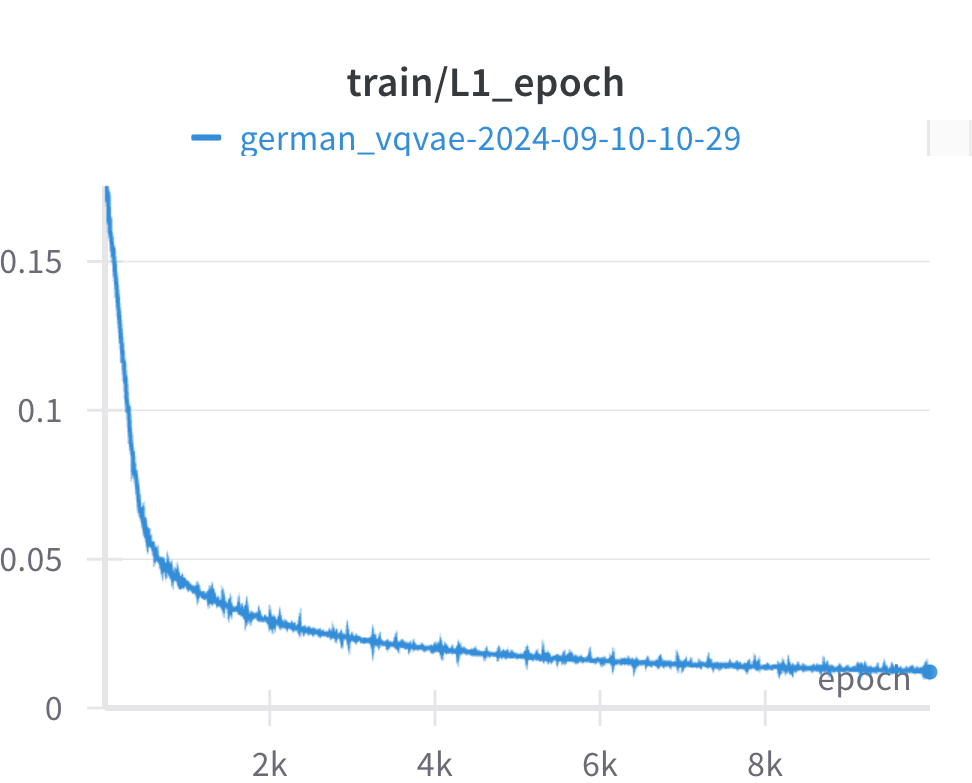
\includegraphics[width=\linewidth]{detailed_engineering/German VQVAE/charts/train_l1.png}
\caption{}
\endminipage\hfill
\minipage{0.49\textwidth}
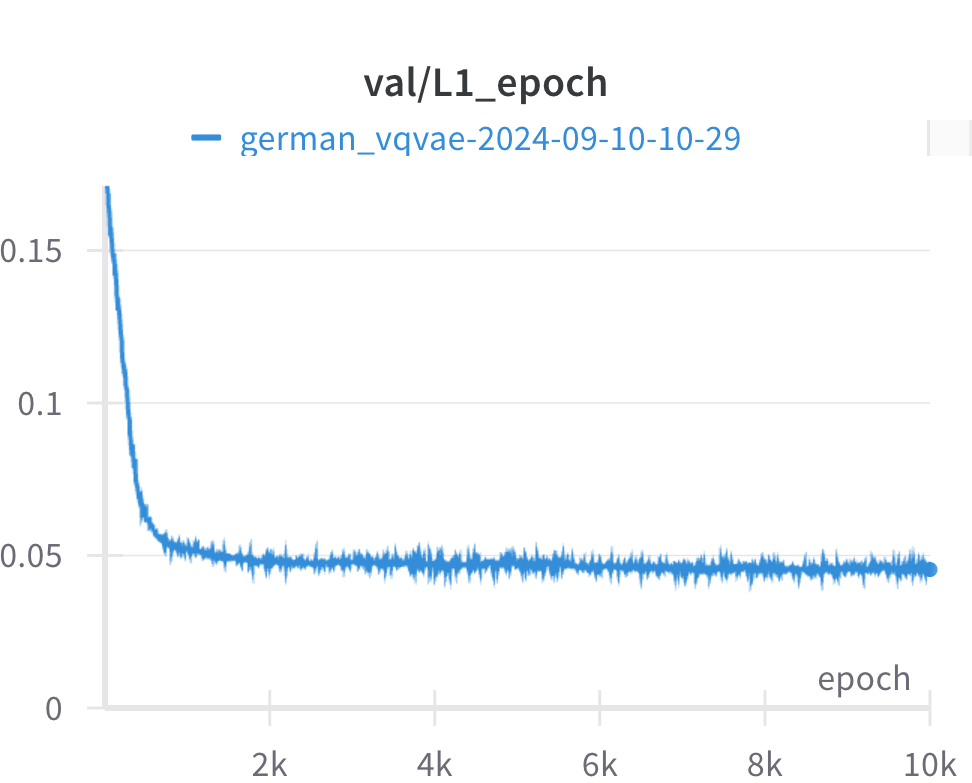
\includegraphics[width=\linewidth]{detailed_engineering/German VQVAE/charts/val_l1.png}
\caption{}
\endminipage
\end{figure}

\begin{figure}[H]
\minipage{0.49\textwidth}
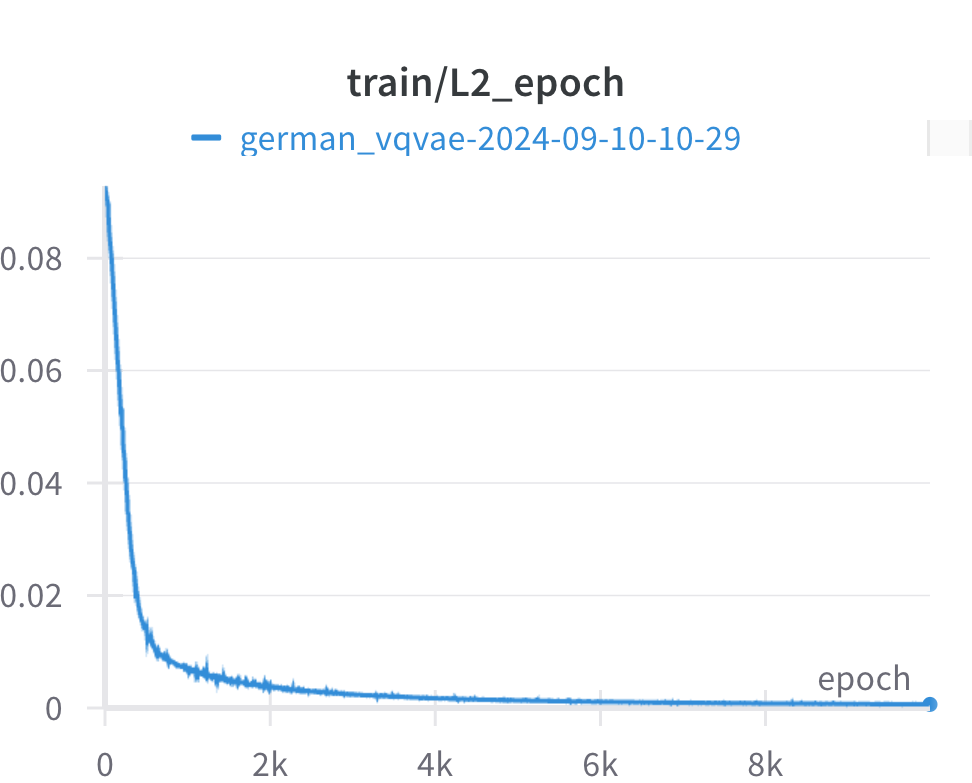
\includegraphics[width=\linewidth]{detailed_engineering/German VQVAE/charts/train_l2.png}
\caption{}
\endminipage\hfill
\minipage{0.49\textwidth}
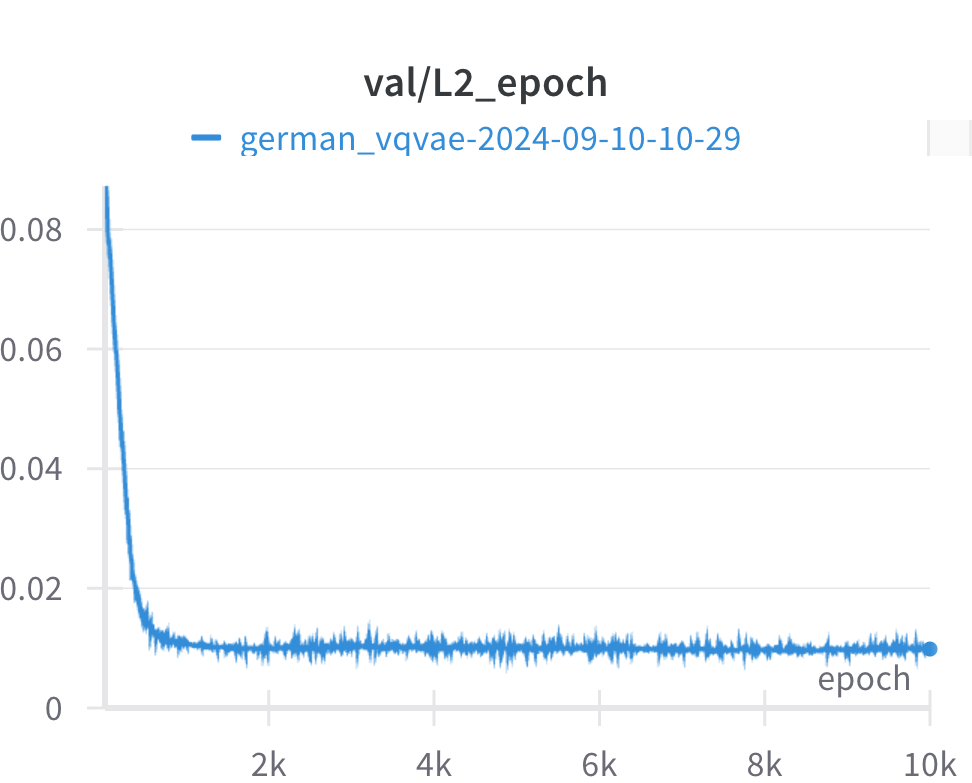
\includegraphics[width=\linewidth]{detailed_engineering/German VQVAE/charts/val_l2.png}
\caption{}
\endminipage
\end{figure}

\begin{figure}[H]
\minipage{0.49\textwidth}
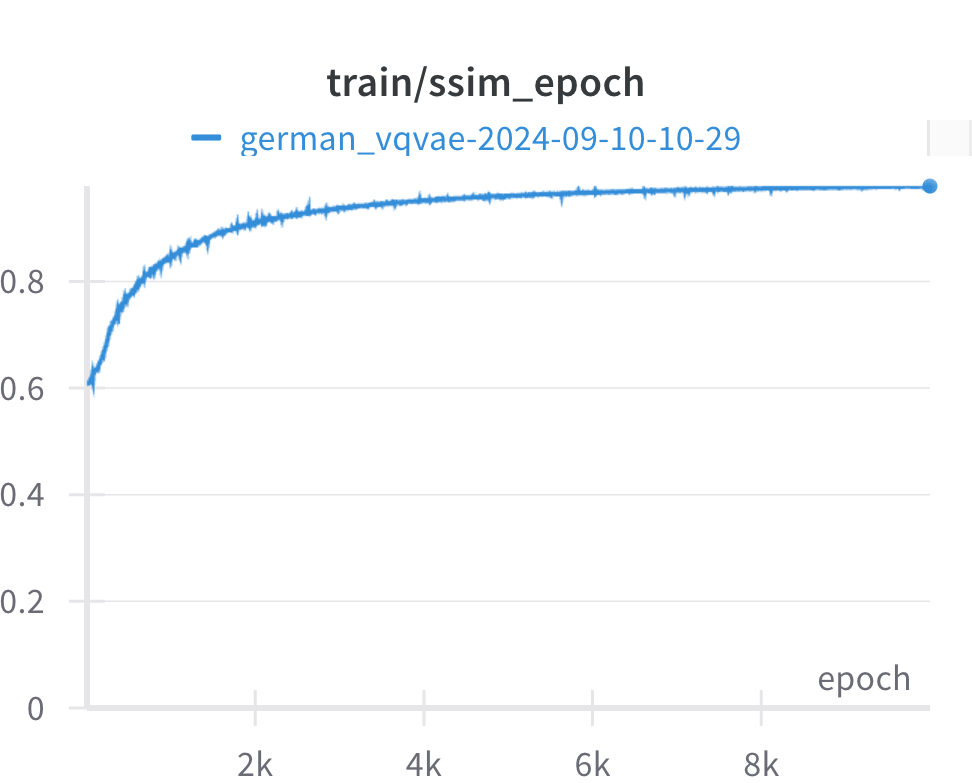
\includegraphics[width=\linewidth]{detailed_engineering/German VQVAE/charts/train_ssim.png}
\caption{}
\endminipage\hfill
\minipage{0.49\textwidth}
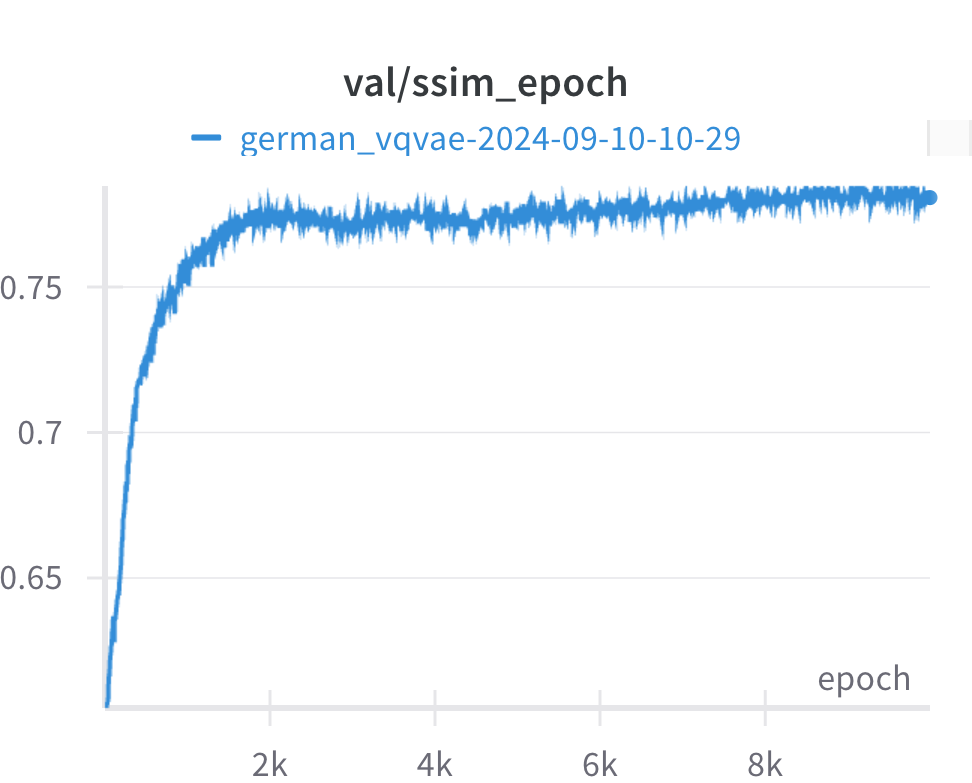
\includegraphics[width=\linewidth]{detailed_engineering/German VQVAE/charts/val_ssim.png}
\caption{}
\endminipage
\end{figure}




\paragraph{Results}\mbox{}\\

\begin{figure}[H]
    \centering
    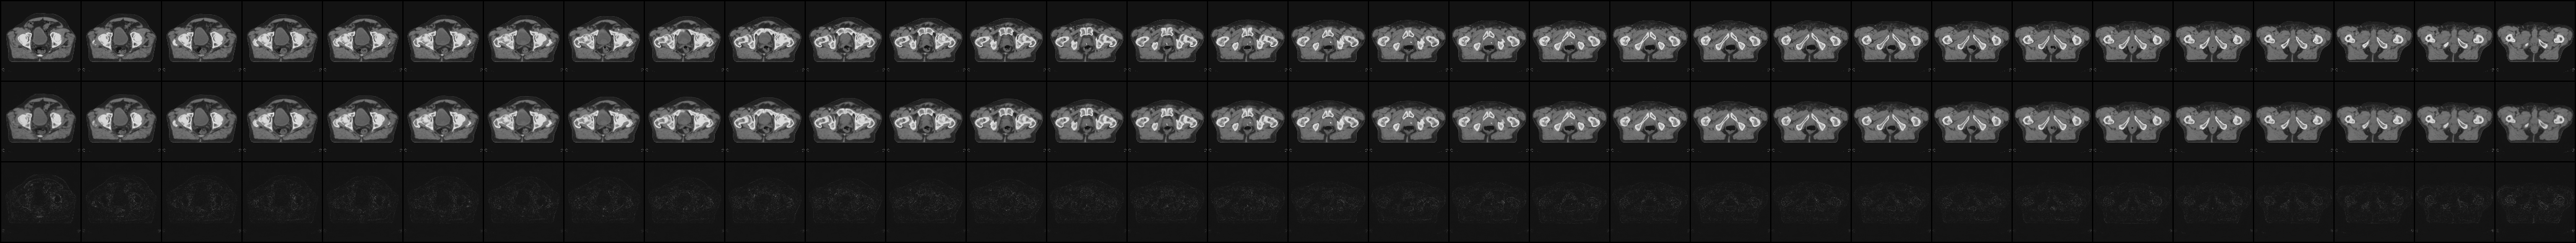
\includegraphics[width=\linewidth]{detailed_engineering/German VQVAE/charts/best_german_vqvae.png}
    \caption{The best quality reconstruction achieved. Epoch 8499, step 10540. Top - input, middle - reconstruction, bottom their difference}
    \label{fig:german_vqvae_best}
\end{figure}

